\section{Data Dissemination in ICN}\label{pubsub}
Publish/Subscribe model is a comment approach in IoT system for resource sharing and management. In traditional IP network, most of the IoT platforms provide a centralized server to aggregate all IoT device resources, publish them to the web portal,and manage the subscribing membership. The subscriber may need to retrieve the sensor data from the server. Such centralized architecture no doubt can benefit the accessibility for each device. However, scalability and bandwidth consumption due to control and data information exchange may be a significant issue, if billions of IoT devices involve. Thus, a decentralized publish/subscribe model might be needed to solve this challenge.

Content-Oriented Pub/Sub System (COPSS)\cite{} achieve an efficient pub/sub capability for CCN. It integrates a push based multicast module with the pull based CCN architecture at the content-centric layer.

\subsection{Pub/sub in MobilityFirst}
To maintain the convenience of traditional centralized Pub/Sub model and reduce the bandwidth consumption, we propose the Pub/Sub model in MF IoT platform.In order satisfy requirement of different applications, we provide two communication model--push and pull mode for sensor data retrieval in MobilityFirst.

\subsubsection{Basic Push Mode}
In many IoT applications, data transmission is event-driven, where sensor or sink tends to update itself to the server as specific event is detected.For instant, smoke sensor will be triggered only when smoke is detected, it needs to update the monitoring application in the shortest time. In this case, a push-based low latency data transmission approach is necessary.    As what we introduce above, Configuration Service registers the all devices in the IoT server, where subscription membership is managed. Taking security and MobilityFirst multicast into account, we introduce a new type of GUID -- Subscription GUID(sGUID) here. Besides identifying devices, application and content in the MF network, GUID can also be used to establish a subscription relationship. 

When a application subscribes to a web service that providing sensor resources over the IoT server, a sGUID will be assigned to it and listened as a destination GUID. Single Subscription GUID can be assigned to multiple applications, if they subscribe to the same sensor resource. The sink of the subscribed sensor will be notified with the Subscription GUID.Without knowing the GUID of application,sink set this sGUID into the destination GUID field in a MF header, and begin to send sensor data. Taking advantage of GSTAR\cite{} routing protocol and host protocol stack\cite{} in MF, whenever a receiver announce a new GUID being listened, its MF access router performs a GNRS insert and add it to local routing table. Therefore, if different clients announce they listen at the same sGUID, the nearest MF router performs a multicast so that all of them can receive data from source sensor. For example, shown as Figure~\ref{fig:pubsub}, application $GUID=789$ subscribes to sensor $GUID=123$ on IoT server. $sGUID=456$ will be assigned to both the sink and application. At the sink side, sGUID will be set as destination GUID, whenever sensor updates to the sink, this data will be sent to $sGUID=456$. The MF access router will be updated if host announces a new GUID is added to the listening list. Since GUID is consistent in the network, such approach utilize locator/identifier split mechanism of MF, where locator here is the GUID of the MF access router. Mobility of both the client and application running on it can be handled properly.   
%update the figure to show the sensor,table, and routing table. 
\begin{figure}
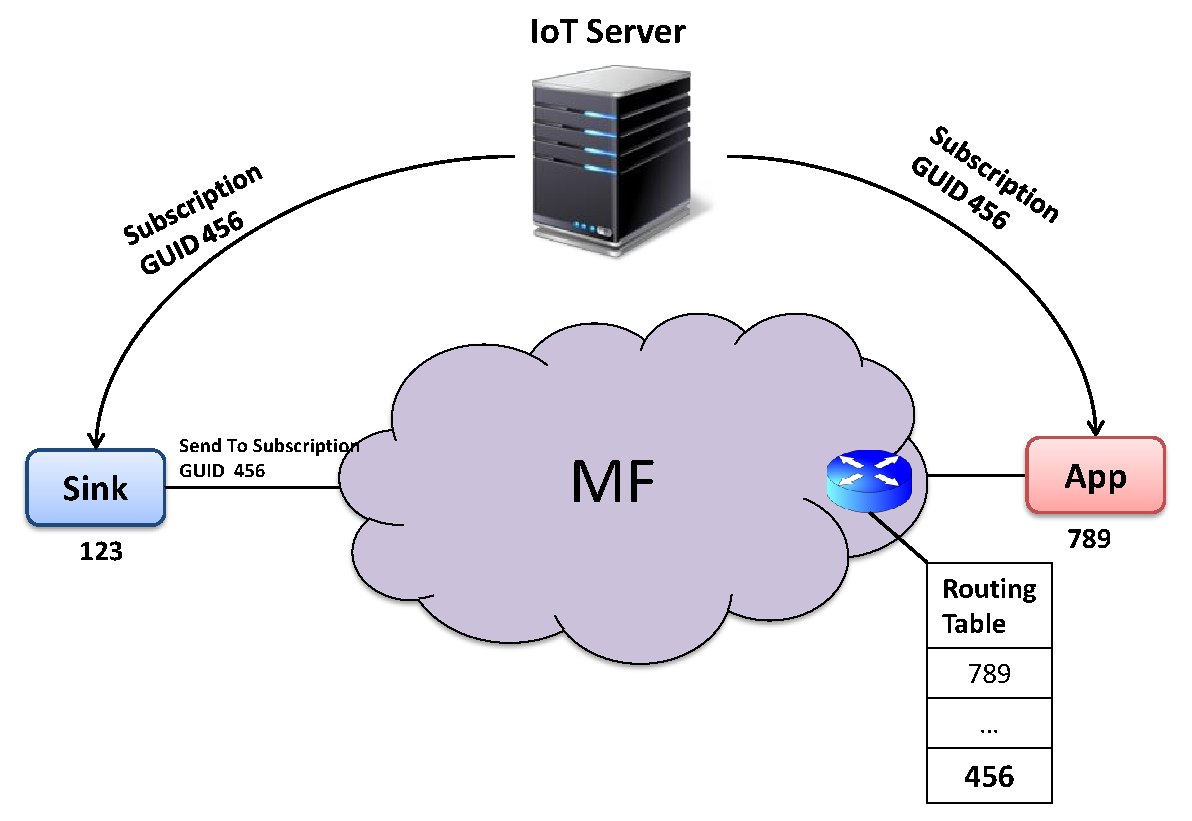
\includegraphics[width=3.00in,height=2.00in]{pubsub_push.eps}
\caption{Basic Push Mode on MF IoT}
\label{fig:pubsub}
\end{figure}

\subsubsection{On Demand Pull Mode}
In ICN architecture, where we include the concept of data consumer and producer, data transmission is on-demand--it is driven by the interest from data consumer, and data producer respond per request. Instead of a single sensor, application sometimes tends to subscribe to a certain service, which may include a group of sensors.Therefore, a sensor data retrieval method in MF is proposed to enable application pulling sensor data based on certain criteria or context.

Besides basic one-to-one data request and reply communication, we would like to introduce a mechanism where multiple sensor objects can be access via one sink node, so that many-to-one or one-to-many capability can be achieved. To associate a group of sensor with a subscriber application, we can make use of the Subscription GUID, in order to reduce the complexity of the information for the subscriber application. In order words, it can send data request to multiple sensors on multiple sinks by single Subscription GUID. However, the question is when the sink receive the message via the a single sGUID, how can it learn which sensors that application want exactly? IoT server needs to provide more hints to the sink node. Shown as Figure~\ref{}, we establish a relationship between the sensors and the application in the IoT server. Similar to the basic push mode we discuss above, IoT server assigns a message with sGUID followed by multiple sensor GUIDs which is in the subscription, so that sink node can understand the exact sensor objects to access. Since every request packet contains the GUID of the applicaton, sink nodes can respond to it without querying any third party service. 
%We assume that IoT server already knows  the service GUID and locator GUID(GUID of the router), which already contain certain context information from name assignment service.
% For example, since sink node is relatively stationary and aggregates limited types of sensor,the service GUID can represent the environment sensing, as well as the identifier for the sink. IoT server use the service GUID and router GUID to look up in the GNRS server. In respond, two lists of GUID will be sent back to IoT server. After comparing these two lists,IoT server can obtain the desired group of sensor GUIDs. Furthermore, 

%make a figure for IoT server finding sensor guid andt sink application pulling data from sink node.
\begin{figure}
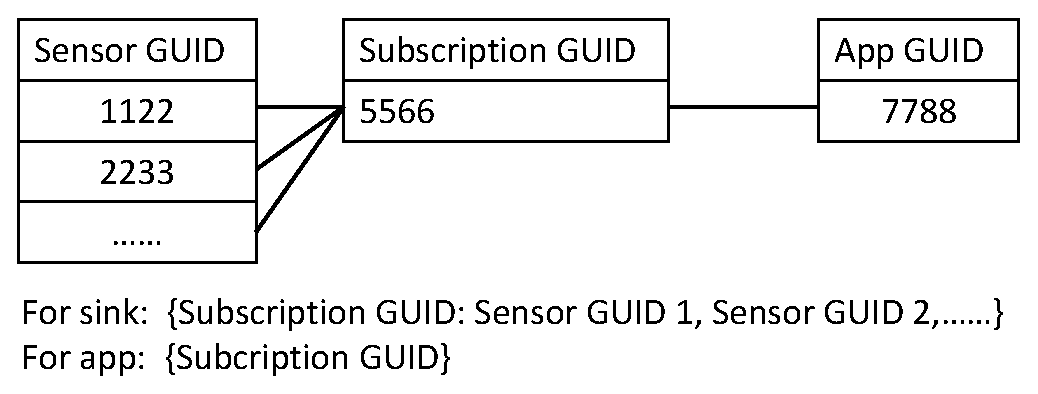
\includegraphics [width=3.00in,height=1.30in]{two_step_pull.eps}
\caption{Mapping Relationship}
\end{figure}